\documentclass[12pt, bibliography=totoc]{scrartcl}
%\setkomafont{caption}{\small\bfseries\selectfont}
%\setkomafont{captionlabel}{\small\bfseries}
\usepackage[headsepline,automark]{scrlayer-scrpage} %Trennlinie an Kopfzeile
%\usepackage{scrheadings}
\clearpairofpagestyles
\lohead{\rightmark}
%\renewcommand{\partmark}[1]{\relax}% \part daran hindern, den Kolumnentitel zu löschen
\ohead[]{\pagemark}
%\ofoot*{\pagemark}
%%Kopfzeile
\usepackage{txfonts} %für times new roman
%\usepackage{helvet} %für arial, dann aber 11pt
\usepackage[a4paper, left=2cm, right=2.5cm]{geometry}
\usepackage[onehalfspacing]{setspace}
%\usepackage{apacite}
\usepackage{caption}
\captionsetup{labelfont={scriptsize,bf}}
\captionsetup{font={scriptsize,bf}}
\usepackage{wasysym}
\usepackage{mbenotes}
\usepackage{rotating}
\usepackage{framed}
%\usepackage{amsmath}
%\usepackage{amssymb}
\usepackage{float}
%\usepackage{caption}
\usepackage[T1]{fontenc}
\usepackage[utf8]{inputenc}
%\usepackage{todonotes}
\usepackage{enumitem}
%\uespackage{caption}
%\usepackage[bf]{caption}
%\renewcommand{\captionfont}{\small\slshape}
%\renewcommand{\figurename}{Abb.}
%\renewcommand{\thefigure}{\arabic{section}.\arabic{figure}}
%\makeatletter \@addtoreset{figure}{section} \makeatother
%\captionsetup[figure]{skip=1pt}
\usepackage{tabularx}
\usepackage{pdfpages}
\usepackage{array}
\usepackage{hyperref}
\usepackage{threeparttable} %fußnoten unterhalb tabelle
\usepackage{booktabs} % fuer schone Tabellen
\usepackage{rotating} % um tabellen auf quer drehen zu koennen http://www.golatex.de/kann-man-tabellen-im-querformat-darstellen-t2003.html
%\newcolumntype{C}[1]{>{\centering\arraybackslash}p{#1}} %Spalten mit fester breite zentriert
%\newcolumntype{L}[1]{>{\raggedright\arraybackslash}p{#1}} %Spalten mit fester breite linksbündig
%\newcolumntype{Y}{>{\small\raggedright\arraybackslash}X}
%\newcolumntype{C}{>{\small\centering\arraybackslash}X}
\usepackage{graphicx}
%\usepackage[german]{babel}
\usepackage{typearea}
%für Randbemerkungen, sehr nützlich:
\usepackage{xargs}                      % Use more than one optional parameter in a new commands
\usepackage[pdftex,dvipsnames]{xcolor}
\usepackage[colorinlistoftodos,prependcaption,textsize=tiny]{todonotes}
\newcommandx{\unsure}[2][1=]{\todo[linecolor=red,backgroundcolor=red!25,bordercolor=red,#1]{#2}}
\newcommandx{\change}[2][1=]{\todo[linecolor=blue,backgroundcolor=blue!25,bordercolor=blue,#1]{#2}}
\newcommandx{\info}[2][1=]{\todo[linecolor=OliveGreen,backgroundcolor=OliveGreen!25,bordercolor=OliveGreen,#1]{#2}}
\newcommandx{\improvement}[2][1=]{\todo[linecolor=Plum,backgroundcolor=Plum!25,bordercolor=Plum,#1]{#2}}
\newcommandx{\thiswillnotshow}[2][1=]{\todo[disable,#1]{#2}}
% erklaerung siehe hier http://tex.stackexchange.com/questions/9796/how-to-add-todo-notes

%hat prima funktioniert:
\usepackage[style=apa,backend=biber]{biblatex}
\usepackage[american,ngerman]{babel}
\DeclareLanguageMapping{ngerman}{ngerman-apa}
\usepackage[babel,german=guillemets]{csquotes}
%\bibliographystyle{apacite}
%nach part fängt section wieder mit eins an alte Gestaltung
%\makeatletter
%\@addtoreset{section}{part}
%\makeatother
%\renewcommand*{\partformat}{\thepart}{}
%\renewcommand*{\partheadmidvskip}{\nobreak\enskip}
\bibliography{/Users/Mama/Dropbox/Biblio/library}
%\bibliography{/Users/iNge/Dropbox/Biblio/library}
%\bibliography{library}




\begin{document}
\renewcommand\finalandcomma{\addcomma}

\begin{titlepage}
\thispagestyle{empty}
\begin{center}
\color{blue}\Large{Fernuniversität Hagen}\\
\end{center}


\begin{center}
\Large{Bildung und Medien: eEducation}
\end{center}
\begin{verbatim}



\end{verbatim}
\begin{center}
\textbf{\Large{Kommentierte Bibliographie zum Thema Online-Lernen}}
\end{center}
\begin{verbatim}

\end{verbatim}
\begin{center}
\textbf{Fakultät Kulturwissenschaften}
\end{center}
\begin{verbatim}










\end{verbatim}

\begin{flushleft}
\begin{tabular}{lll}
\textbf{Studiengang:} & & MA Bildung und Medien: eEducation\\
& & Modul 2: Anwendungsbezogene Bildungsforschung\\
& & \\
& & \\
\textbf{eingereicht von:} & & {\color{magenta} Inge Koch-Meinass \flq{}ingekoch@mac.com\frq{}}\\
& & {\color{magenta}Matrikelnr.: 123456 }\\
& & \\
\textbf{eingereicht am:} & & 06. November 2015\\
& & \\
& & \\
%\textbf{Betreuer:} & & Herr Prof. Dr. J. A. Müller
\end{tabular}
\end{flushleft}

% das ist wohl jetzt das Ende des Dokumentes
\end{titlepage}


%% das Papierformat zuerst
%\documentclass[a4paper, 11pt]{article}

% deutsche Silbentrennung
%\usepackage[ngerman]{babel}
%\usepackage{color} \color{blue}
% wegen deutschen Umlauten
%\usepackage[utf8]{inputenc}

% hier beginnt das Dokument
%\begin{document}

\begin{titlepage}
\thispagestyle{empty}
\begin{center}
\color{blue}\Large{Fernuniversität Hagen}\\
\end{center}


\begin{center}
%\Large{Bildung und Medien: eEducation}
\end{center}
\begin{verbatim}



\end{verbatim}
\begin{center}
\textbf{\Large{Kommentierte Bibliographie zum Thema Online-Lernen}}
\end{center}
\begin{verbatim}

\end{verbatim}
\begin{center}
%\textbf{im Studiengang Wirtschaftsinformatik}
\end{center}
\begin{verbatim}











\end{verbatim}

\begin{flushleft}
\begin{tabular}{lll}
\textbf{Studiengang:} & & MA Bildung und Medien: eEducation\\
& & Modul 2: Anwendungsbezogene Bildungsforschung\\
& & \\
& & \\
\textbf{eingereicht von:} & & {\color{magenta} Inge Koch-Meinass \flq{}ingekoch@mac.com\frq{}}\\
& & {\color{magenta}Matrikelnr.: 9650962 }\\
& & \\
\textbf{eingereicht am:} & & 06. November 2015\\
& & \\
& & \\
%\textbf{Betreuer:} & & Herr Prof. Dr. J. A. Müller
\end{tabular}
\end{flushleft}

% das ist wohl jetzt das Ende des Dokumentes
\end{titlepage}

\listoftodos[Gesammelte Unklarheiten]
\tableofcontents
%\listoftables
\setcounter{page}{1}
%\thispagestyle{empty}
\pagebreak

\section{Einleitung}\label{einleitung}

\improvement{Pisa abschneiden machte es erforderlich usw.. Hier Holzkamp konkret}
\glqq Das weltweit verfügbare Wissen verdoppelt sich zurzeit alle vier
bis fünf Jahre. Der amerikanische Soziologe Richard Sennet (1998)
erwartet, dass ein amerikanischer College Student in seinem Berufsleben
elf Mal die Stelle wechselt und dreimal die Basis seines Wissens
komplett austauscht \parencite[138]{Ehlers2002}.\grqq{} Vor diesem
Hintergrund kommt der beruflichen Weiterbildung eine immer größere
Bedeutung zu, den beruflichen Anforderung gerecht zu werden, erfordert
die Bereitschaft zu lebenslangem Lernen. Mit dem Zuwachs an Veränderung
in Organisationen und der damit verbundenen Anforderung „am Ball zu
bleiben`` gilt es Lernkonzepte zu finden die modernen
konstruktivistischen Lerntheorien einerseits und beruflichem Lernen von
Erwachsenen andererseits gerecht werden. Das immer größere Lernpensum,
kann nicht ausschließlich in Präsenzveranstaltung gelehrt werden,
sondern viel mehr gilt es von Zeit und Ort unabhängige Lernmöglichkeiten
zu schaffen. Digitale Lernplattformen leisten hier einen wichtigen
Beitrag und können je nach didaktischer Aufbereitung,
selbstorganisiertes, konstruktivistisches und damit nachhaltiges Lernen
fördern. Die vorliegende Arbeit befasst sich mit der Evaluation einer
beruflichen Weiterbildung, die als Blended Learning Kurs für
FrühpädagogInnen
\footnote{Der Begriffe FrühpädagogInnen, schließt alle im Kitabereich tätigen Fachkräfte ein}
konzipiert wurde. Inhalt der Weiterbildung ist das kennenlernen und
umsetzen können des Early-Excellence Konzept, ein Ansatz mit dem
Bildungs- und Orientierungspläne der Bundesländer in den
Kindertagesstätten konzeptionell verankert werden können. Mit Hilfe
eines standardisierten Fragebogens wird versucht, den durch die
Weiterbildung gewonnen, selbst eingeschätzten Zuwachs an
Handlungskompetenz zu bestimmen. Es wird einmal das
Weiterbildungsangebot insgesamt und zum anderen der Einfluss der
digitalen Lernplattform betrachtet.

\section{Theorierahmen}\label{theorierahmen}

Der der Untersuchung zugrundeliegende Theorierahmen umfasst die Themen
Erwachsenenbildung im Blended Learning Verfahren und daraus
resultierender Zuwachs an Handlungskompetenz.

\subsection{Erwachsenenbildung}\label{erwachsenenbildung}

Das Lernen Erwachsener unterliegt besonderen Gegebenheiten, die hier
nachfolgenden beschrieben werden. Lernen im Erwachsenenalter ist
überwiegend gekennzeichnet durch Anschlusslernen. Der Erwachsene knüpft
beim Lernen an Bekanntes an, Lernen erfolgt konstruktivistisch und
subjektorientiert: „Erwachsene lassen sich in der Regel nicht belehren
oder aufklären, Wahrheiten lassen sich nicht linear vermitteln.
Erwachsene haben ihren eigenen Kopf, machen sich ihre eigenen
Gedanken\ldots`` \parencite[15]{Siebert201408}. Dies unterstreicht
einmal mehr, dass Lernen nicht hergestellt, sondern nur vom Individuum
selbst vollbracht werden kann \parencite{Faulstich2012}.

In subjektorientierten Lerntheorien z.B.: \parencite{Holzkamp2004} wird
Lernen beschrieben als eine Erweiterung von Handlungsfähigkeit und nicht
als Anhäufung von Wissen. Holzkamp prägte den Begriff des „expansiven
Lernens'', der ausdrücken soll, dass „intentionales, d.h. absichtliches
und geplantes Lernen nur dann zustande kommt, wenn das Lernsubjekt
selbst entsprechende Gründe dafür hat`` {[}\ldots{]}
\parencite[29]{Holzkamp2004}. Nach Holzkamp kommt es dann zum Lernen,
wenn das „Subjekt in seinem normalen Handlungsvollzug auf Hindernisse
oder Widerstände gestoßen ist{[}\ldots{]}.`` Im vorliegenden Fall ist
das „Hindernis`` die Einführung von Bildungs- und Orientierungsplänen in
Kitas, die es erforderlich machen den „normalen Handlungsvollzug`` zu
verändern. Diese Problematik kann nicht mit dem vorhandenen Wissen und
den vorhandenen Fähigkeiten gelöst werden, sondern erfordert das
„Einschalten einer Lernschleife`` \parencite[29]{Holzkamp2004}. Diese
Lernschleife wird mit der hier beschriebenen Weiterbildungsmaßnahme
unter Berücksichtigung, dass es unmöglich ist, Inhalte passiv in Köpfe
füllen zu können \parencite[12]{Faulstich2012}, gedreht. Schon 1993
verweist Holzkamp in seinem Buch Lernen auf die Notwendigkeit den Lerner
in den Mittelpunkt zu stellen, verweist auf den Lehr-Lern-Kurzschluss
und übt scharfe Kritik am vorherrschenden Schulsystem. Während die
didakische Umsetzung der Subjektorientierung in Schulen wenig
aufgegriffen wird, ist sie in der beruflichen Erwachsenenbildung eher
gängig \parencite{grotluschen2005expansives}.
\textcite[138]{ehlers2011qualitat} beschreibt vier Gründe für den immer
größer werdenden Stellenwert des Lerners in Weiterbildungsmaßnahmen:
\emph{Ökonomische} Gründe liegen vor, weil die Lerner Weiterbildung oft
selbst finanzieren und/oder die Weiterbildung in der Freizeit machen.
\emph{Pädagogisch-didaktische} Gründe liegen im Wandel zu
konstruktivistischen Lerntheorien, die eine Subjektorientierung
bedingen. \emph{Gesellschaftlich} ist die Entwicklung hin zur
Wissensgesellschaft zu betrachten und die Entwicklung hin zum
\emph{eLearning} als Lernform, dass per se den Lerner als Akteur
einbezieht. Auch die hier beschriebene Weiterbildungsmaßnahme orientiert
sich an den Grundlagen des subjektorientierten Lernens und vor dem
Hintergrund, dass die Teilnehmer sehr individuelle Lernzugänge haben und
letztlich nur selbst ihre Handlungsfähigkeit erweitern können. Die
Inhalte bestehen weniger in Vermittlung von Faktenwissen als vielmehr in
der Anknüpfung von bereits Erlebten in Form von Biographiearbeit und der
Berücksichtigung der jeweils unterschiedlichen Kontextbezügen. Dies wird
in den Präsenzphasen, als auch mit der Lernplattform beispielsweise
dadurch umgesetzt, dass die Lerner zugleich auch Lehrende sind, Inhalte
aktiv mitgestalten und wiederum der Gemeinschaft zur Verfügung stellen.

Vor diesem Hintergrund wird in der vorliegenden Arbeit der „Lernerfolg``
eben als solche Erweiterung von Handlungsfähigkeit, in Form von Zuwachs
an Handlungskompetenz gemessen.

\subsection{Blended Learning}\label{blended-learning}

Im folgenden soll der Begriff des Blended Learning und was im Rahmen
dieser Arbeit darunter zu verstehen erläutert werden. Direkt übersetzt
bedeutet Blended Lerning „vermischtes Lernen``. Das heißt es handelt
sich bei dieser Lernform um ein Lehr-Lernsetting, dass sowohl
klassisches Face-to-Face-Lernen, als auch eLearning beinhaltet. Die
verschiedenen Lernangebote stehen sich nicht als entweder oder
gegenüber, sondern als sich ergänzend.
\texcite[3]{kerres2001multimediale} betont „dass die besondere Qualität
und auch Effizienz eines Lernangebotes vor allem in der Kombination von
Elementen unterschiedlicher methodischer und medialer Aufbereitung zum
Tragen kommt``. \textcite[45]{ehlers2011qualitat} merkt kritsch an, dass
der Begriff nicht vermischtes Lernen meint, sondern, dass es um eine
Mischung von Methoden mit denen gelernt wird, geht. „Blended Learning
strebt die Optimierung von Lernprozessen zur Erreichung individueller
Lernziele unter der Nutzung aller dafür geeigneter Lehr-Lernmethoden
an`` \parencite[46]{ehlers2011qualitat}. Blended Learning Konzepte gibt
es schon seit vielen Jahren und sie werden sowohl in Schulen und
Hochschulen , als auch in beruflichen Weiterbildungsmaßnahmen
eingesetzt. Elearning Angebote wurden in Deutschland nur sehr zögerlich
angenommen, es überwiegen in weiten Bereichen noch traditionelle
Lernformen. Aus dieser Situation heraus bot sich das Blended Learning
als Lernform an, da es traditonelle und moderne, digitale Lernformen
miteinander verbindet \parencite{Maihack2015}. Für den Einsatz von
Blended Learning sprechen nach \textcite{thomas2000evaluating}
zahlreiche Gründe: * Orts- und Zeitunabhängigkeit

\begin{itemize}
\item
  Leichte Aktualisierbarkeit
\item
  Lerner haben viel Kontrolle: sie können wählen, was sie wann lernen,
  können auf bereits durchgenommenes Material zugreifen usw.
\item
  Viele Möglichkeiten der Interaktion
\item
  Es können beliebig viele Personen am Kurs teilnehmen
\end{itemize}

Die Form des hybriden Lernens erlaubt es, Vorteile von digitalem Lernen
(selbstorganisiert, zeit- und ortsunabhängig, ) und Vorteile von
traditionellem Lernen (sich kennen lernen, Gruppen bilden, Motivation
\ldots) zu kombinieren \parencite{Zumbach2010}. Für die Gestaltung eines
eLearning Angebotes auf der Grundlage einer konstruktivistischen
Lerntheorie, ist es notwendig den Lernenden die Möglichkeit der
Eigentätigkeit, Formen des sozialen Austausches, Möglichkeiten zur
Bearbeitung komplexer Probleme usw. einzuräumen
\change{woher ist das? Zitat}. Letzlich soll dieses Lernarrangement
selbstorganisiertes und reflexives Lernen ermöglichen.

Es sei angemerkt, dass es sowohl verschiedene Begriffe, als auch
verschiedene Definitionen von Blended Learning gibt. Neben Begriffen wie
integrated Learning, flexible Learning usw. wird es im deutschen
Sprachraum oft auch als \enquote{Hybrid Teaching} benannt
\parencite{Oliver2005}\{kerres2001multimediale\}. In der vorliegenden
Arbeit meint Blended Learning, die sich ergänzende Kombination von
verschiedenen Medien, nämlich Präsenzlernen in Form von Wochendseminaren
und eLearning in Form einer Moodle-Lernplattform.

\subsection{Handlungskompetenz}\label{handlungskompetenz}

Die Qualität der hier beschriebenen Weiterbildung wird auf der Ebene des
Ergebnisses evaluiert. Wird wie oben beschreiben der Lerner in den
Mittelpunkt gerückt, kann der Lernerfolg nur der Zuwachs an
Handlungskompetenz sein. \parencite[4]{Ehlers2002}. Gemessen werden
nicht Leistungsresultate, sondern vielmehr die Fähigkeit bzw.
Disposition neue, kreative Lösungen hervorzubringen, die Messung des
Kompetenzzuwachses orientiert sich am Einzelnen und entspricht somit der
Subjektzentrierung des vorgestellten Lernarrangements
\parencite{ErpenbeckRosenstiel200305}. Handlungskompetenz meint hier die
„Fähigkeit in einer komplexen Welt gestaltend mit der Umwelt agieren zu
können`` \parencite[4]{Ehlers2002}.

Die Handlungskompetenz setzt sich nach
\textcite{ErpenbeckRosenstiel200305} aus verschiedenen Kompetenzen
zusammen, die nach \textcite{ErpenbeckRosenstiel200305} und
\autocite{Braun2008} wie folgt zusammengefasst und beschrieben werden
können:

\begin{enumerate}
\def\labelenumi{\arabic{enumi}.}
\item
  Personale Kompetenzen: Diese Kompetenz beschreibt z.B.: die Fähigkeit
  selbstorganisiert zu handeln, sich selbst einschätzen zu können,
  Motive und Werte des Handelns.
\item
  Fachkompetenz: Beschreibt Kenntnisse, Verständnis,
  Anwendungsfähigkeiten und Analysefähigkeiten der Lernenden.
\item
  Methodenkompetenz: Beherrschung von Arbeitstechniken,
  Planungsvermögen, Vermögen Wissen sinnorientiert einsetzen zu können
\item
  Sozialkompetenz: Dies beinhaltet sowohl die Kommunikations- als auch
  die Kooperationsfähigkeit und beschreibt die Fähigkeit eigene und
  gemeinsame Ziele in Zusammenarbeit erreichen zu können.
\end{enumerate}

\section{Operationalisierung}\label{operationalisierung}

Der nicht direkt messbare Zuwachs an Handlungskompetenz, macht es
notwendig Indikatoren zu bilden, die den Lernerfolg abbilden können. Für
die einzelnen Kompetenzen muss also gefragt werden, woran man den
Zuwachs an dieser erkennen kann. Den Zuwachs an Personalkompetenz kann
zum Beispiel über Freude, Interesse, intensive Beschäftigung mit dem
Thema usw. erfasst werden. „Ein Indikator ist ein direkt beobachtbarer
Sachverhalt, der durch Korrespondenzregeln mit dem nicht direkt
beobachtbaren Sachverhalt verknüpft wird {[}\ldots{]}``
\parencite[85]{Kromrey2009}. Die Korrespondenzregeln beschreiben wie eng
die zugrundeliegenden Indikatoren, mit dem tatsächlich zu messenden
Sachverhalt korreliert sind. Da es sich im vorliegenden Fall um
schlussfolgernde Indikatoren (es wird von nicht direkt beobachtbaren
Sachverhalten auf eine bestimmte Merkmalsausprägung geschlossen)
handelt, ist der Zusammenhang zwischen Indikator und der zu
untersuchenden Kompetenz nicht empirisch überprüfbar, sondern
„{[}\ldots{]} auf den Glauben an die Richtigkeit {[}\ldots{]}``
\parencite[166]{Kromrey2009} angewiesen. Wie bereits beschrieben wird
der Erfolg der hier beschriebenen Weiterbildung an selbsteingeschätzten
Kompetenzen gemessen. Der vorliegenden Arbeit liegt das Messinstrument
von \textcite{Braun2008} zugrunde. Die Autoren haben dieses Instrument
entwickelt, um den „subjektiven Erwerb von Kompetenzen durch den Besuch
einzelner Lehrveranstaltungen {[}messen zu
können{]}``\parencite[30]{Braun2008a}. Der Berliner
Evaluationsinstrument besteht aus 26 Items und drei Filterfragen. Die
Fragen zur \emph{Fachkompetenz} versuchen den Kompetenzzustand zu
erfassen, z.B.:„Ich kann wichtige Begriffe der Weiterbildung
wiedergeben\enquote{, während die weniger wissensspezifischen
Kompetenzen (\emph{Personal-, Sozial-, und Methodenkompetenz}) explizit
den Zuwachs der Kompetenz erfragen, z.B.: „In Folge dieser
Weiterbildung, kann ich meine Arbeit besser strukturieren}.

\subsection{Inhalte der Weiterbildung}\label{inhalte-der-weiterbildung}

Das schlechte Abschneiden deutscher Kinder bei der PISA-Studie 2001
führte unter anderem dazu, dass in Kindergärten und Kindertagesstätten
Bildungs- und Orientierungspläne eingeführt. Die Umsetzung der Pläne
erfolgte nach sehr unterschiedlichen Ansätzen: „Bildungs- und
Lerngeschichten`` \parencite{leu2007bildungs}, „Infans``
\parencite{laewen2011infans} und vielen mehr. In der zu evaluierenden
Weiterbildung wird den Teilnehmern das EEC-Konzept
\parencite{hebenstreit2007early} näher gebracht. Ziele der Weiterbildung
sind zum einen Fachwissen über den Ansatz zu gewinnen, zum anderen
sollen die Teilnehmer, aber auch Methoden der Umsetzung kennen lernen.
Nach der Absolvierung des Blended Learning Kurses und dem Erhalt des
Titels „EEC-Berater`` sollen die Teilnehmer auch in der Lage sein, als
Multiplikatoren den Ansatz weiterzuvermitteln. Die Weiterbildung
erstreckt sich über 12 Monaten innerhalb derer sechs Präsenzmodule
(teilnahmepflicht) zu absolvieren sind.

\subsection{Aufbau der Lernplattform}\label{aufbau-der-lernplattform}

Begleitend zu den Präsenzveranstaltung wurde eine auf Moodle basierende
Lernplattform eingerichtet. Moodle wurde 2000 von Martin Dougiamas, vor
allem als Möglichkeit konstruktivistisches online-Lernen zu ermöglichen,
entwickelt \parencite{dougiamas2002interpretive}. Die Plattform ist,
entsprechend den Präsenzveranstaltungen, modular aufgebaut. Die
Lernplattform beinhaltet zum Einen von Handouts über Präsentationen bis
hin zu den Protokollen eine Fülle an Dateien. Zum anderen werden auch
Aktivitäten, die zum gemeinsamen Lernen einladen, eingestellt. Darunter
fallen Foren, in denen über die Inhalte diskutiert werden oder die
gemeinsame Erstellung eines Glossars. Daneben gibt es noch Fotogalerien,
Lesezeichen, Lernquiz und allgemeine Informationen. Der Besuch der
Lernplattform ist freiwillig - es gibt hier keine verpflichtende
Aufgaben. Allerdings werden Ankündigungen, Termine, Dateien nur über die
Lernplattform zur Verfügung gestellt, was es wiederum erforderlich
macht, sich ab und zu einzuloggen.

\section{Methoden}\label{methoden}

\subsection{Forschungsfrage und
Hypothesen}\label{forschungsfrage-und-hypothesen}

Für die Arbeit wurde folgende Forschungsfrage aufgestellt:

\begin{framed}
Forschungsfrage: Welchen Effekt hat die Teilnahme an einer beruflichen Weiterbildung im Blended Learning Format, auf den selbsteingeschätzten Zuwachs an Handlungskompetenz?
\end{framed}

Um die Frage beantworten zu können werden zwei Hypothesen überprüft:

\begin{framed}
Hypothese 1: Die Teilnahme an der Weiterbildung hat einen positiven Effekt auf den selbsteingeschätzten Zuwachs an Handlungskompetenz.

 Hypothese 2: Der selbsteingeschätzte Zuwachs an Handlungskompetenz, ist um so größer, je intensiver die Lernplattform genutzt wird.
 \end{framed}

\subsection{Studiendesign}\label{studiendesign}

Das Ziel der Studie ist es, die Weiterbildungsmaßnahme inhaltlich, als
auch strukturell zu optimieren. Es wird ein vollstandartisierter
Fragebogen erstellt, der an alle Teilnehmer (20) versandt wird. Außerdem
wird mittels des Fragebogens noch erhoben, wie häufig und zu welchem
Zweck die digitale Lernplattform von den Teilnehmern genutzt wird. Es
handelt sich um eine formative Evaluation, d.h. es ist keine
abschließende Untersuchung, sondern eine Untersuchung, die im laufenden
Prozess durchgeführt wird.

\subsection{Messinstrument}\label{messinstrument}

Für die Messung wird auf der Seite \url{https://www.soscisurvey.de} ein
Onlinefragebogen erstellt. Die Teilnehmer bekommen die Einladung per
Mail zugeschickt, der Fragebogen ist über einen Zeitraum von zwei Wochen
freigeschalten. Die Bearbeitung des Fragebogens dauert etwa 5 Minuten.
Der oben beschriebene Fragebogen enthält zu den einzelnen Kompetenzen
vier bzw. fünf Items. Die Items werden mit einer fünfstufigen
Likertskala (1 = trifft nicht zu; 5 = trifft vollständig zu) abgefragt.

\begin{itemize}
\tightlist
\item
  Methodenkompetenz: besteht aus 4 Items (MK1, MK2, MK3, MK4)
\item
  Fachkompetenz: besteht aus 5 Items (FK1,FK2,FK3,FK4,FK5)
\item
  Personalkompetenz: besteht aus 5 Items (PK1,PK2,PK3,PK4,PK5)
\item
  Kommunikationskompetenz: besteht aus 5 Items (KK1,KK2,KK3,KK4,KK5)
\item
  Insgesamt besteht der Fragebogen aus 26 Items: Mit 18 Items werden die
  Kompetenzen abgefragt und mit 8 Items das Nutzungsverhalten Eine
  ausführliche Zusammenstellung der Items, mit Indikatoren und
  Skalierung findet sich in \improvement{~ref{itemtabelle}}.
\end{itemize}

Für die statistische Auswertung werden die Summenscores der jeweiligen
Items operationalisiert. Diese werden dann entsprechend einer
intervallskalierten Skala behandelt. Dieses Vorgehen ist kritisch zu
betrachten, da eine Rating-Skala streng genommen nur eine Ordinalskala
ist. Die Intervallskala setzt voraus, dass die Unterschiede zwischen den
Stufen, wie zum Beispiel bei einer Temperaturskala, immer gleich groß
sind. Ob dies für eine Ratingskala zutrifft darf hinterfragt werden, da
es aber übliche Praxis ist, solche Ratingskalen intervallskaliert zu
behandeln, wird dies auch für diese Arbeit so übernommen
\parencite[65]{Sedlmeier2013}.

Für eine quantitative Erhebung ist es von entscheidender Bedeutung, dass
die Gütekriterien: Objektivität, Validität und Reliabilität eingehalten
werden \parencite[104]{Hader2015}. Die Objektivität wird in
Durchführungs- Auswertungs- und Interprätationsobjektivität
unterschieden \parencite[70]{Sedlmeier2013}. Die
Durchführungsobjektivität kann hier als gegeben angenommen werden, da es
durch die Online-Befragung zu keiner Beeinflussung durch den
Fragebogenersteller kam. Die Auswertungsobjektivität ist ebenfalls
gegeben, da nur Ratingskalen und keine offene Fragen ausgewertet wurden.
Die Interprätationsobjektivität ist dann besonders hoch, wenn es für die
gewonnen Werte Normen gibt, die das Einordnen der Ergebnisse
erleichtern. Im vorliegenden Fall liegen solche Normen nicht vor, da
noch wenig standardisierten Tests zur Erfassung von Kompetenzen
vorliegen \parencite{Braun2008}.

Die Validität (Gültigkeit der Aussagen) orientiert hier sich an der
Diskussion des zugrundeliegenden, bereits erwähnten Fragebogens
\parencite{Braun2008}. Da es noch wenig Untersuchungen zur Validität bei
Selbsteinschätzung zu Kompetenzen kommt ist die Überprüfung schwierig.
Da aber z.B. bei Untersuchungen zu selbsteingeschätzten
Persönlichkeitsmerkmalen die Validität teilweise sehr hoch ist, wird
davon ausgegangen, „dass Selbstauskünfte einen validen Indikator für
Kompetenzerwerb darstellen.`` \parencite[32]{Braun2008}

Der Fragebogen wurde vor der Verteilung an die Teilnehmer einem Pretest
unterworfen. Die Reliabilität (Genauigkeit mit der ein Merkmal gemessen
wird \parencite[5]{rammstedt2004bestimmung}) wurde mittels dem Cronbachs
alpha Test überprüft wurde \parencite{Wassa}. Es wurden 5 Fragebögen
ausgefüllt und die Ergebnisse für die einzelnen Kompetenzen lagen
zwischen 0.72 und 0.98., was als gut bis sehr gut anzusehen ist
(\textasciitilde{}ref(cronbach)).

\section{Ergebnisse}\label{ergebnisse}

Die Ergebnisse wurden mit dem freien Statistiksoftware R (R - The R
Project for Statistical Computing) ausgewertet. Die gewonnen Daten
wurden als Textdateien aus dem Onlinetool exportiert und in R
eingelesen. Die negativ formulierten Item wurden rekodiert. Es wurden 12
Fragebögen ausgefüllt und ausgewertet. Die Auswertung der Daten erfolgt
univariat und bivariat. Die Ergebnisse werden anhand der Summenwerte der
einzelnen Kompetenzen beschrieben. Die Summenwerte setzen sich aus den
einzelnen Itembatterien zusammen. Die Fachkompetenz und die
Personalkompetenz wurde mit je fünf Items abgefragt. Die Summenwerte
wurden in die Klassen 0-5,5-10,10-15,15-20 und 20-25 eingeteilt. Die
Methodenkompetenz und die Kommunikationskompetenz wurde mit je vier
Items abgefragt und die Ergebnisse wurden wie folgt klassifiziert:
0-4,4-8,8-12,12-16,16-20. Es ergeben sich somit für jede Kompetenz fünf
Klassen, die entsprechend der Likertskala als keinen, geringen,
mittleren, hohen und sehr hohen Kompetenzzuwachs bewertet werden. Die
deskriptiv Statistik zeigt nachfolgend die Häufigkeiten der Antworten
und die Lage- und Streumaße der Einzelkompetenzen, sowie der
Gesamtkompetenz.

\begin{itemize}
\tightlist
\item
  Fachkompetenz
\end{itemize}

\textasciitilde{}\ref{FK} zeigt, dass der Zuwachs an Fachkompetenz mit
mindestens Mittel eingeschätzt wurde (1 Teilnehmer). 75\% der Teilnehmer
schätzen den Zuwachs an Fachkompetenz als sehr hoch ein, zwei Teilnehmer
als hoch. Es gibt keine Teilnehmer, die ihren Zuwachs als nicht
vorhanden oder sehr gering einschätzen.

\begin{figure}[H]
\begin{minipage}{.5\linewidth}
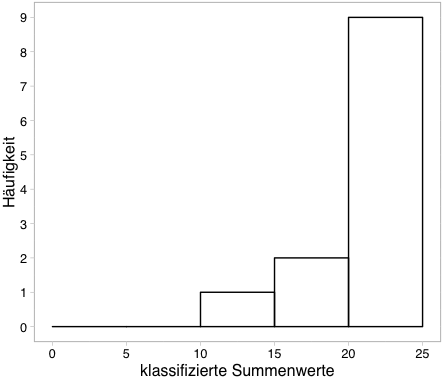
\includegraphics[width=0.8\linewidth]{Anhang/FKHistnn.png}

\end{minipage}
\begin{minipage}{.5\linewidth}
\centering
\raisebox{\depth}
{\begin{tabular}{rrrr}
  \hline
 & absolut & Prozent & kumuliert \\
  \hline
(0,5] & 0.00 & 0.00 & 0.00 \\
  (5,10] & 0.00 & 0.00 & 0.00 \\
  (10,15] & 1.00 & 8.33 & 8.33 \\
  (15,20] & 2.00 & 16.67 & 25.00 \\
  (20,25] & 9.00 & 75.00 & 100.00 \\
   \hline
\end{tabular}

}
%\caption{Häufigkeitstabelle: Fachkompetenz}
\label{tab:defis}
\end{minipage}
\caption{Histogramm und Häufigkeitstabelle der Fachkompetenz}
\label{FK}
\end{figure}

Die Lagemaße der Fachkompetenz (\textasciitilde{}\ref{tab:lFK}) ergeben
einen Mittelwert von ca 21. Dieser sehr hohe Wert entspricht auch dem
Median und dem Modus. Der niedrigste Wert lag bei 14 der höchste Wert
bei 25.

\begin{table}[H]
\centering
\caption{Lage- und Streumaße Fachkompetenz}
\label(tab:lFK)
\begin{tabular}{rrrrrrrr}
  \hline
  N & Minimum & Maximum & Mittelwert & Median & Modus & SD & Varianz \\
  \hline
 12.00 & 14.00 & 25.00 & 20.58 & 21.00 & 21.00 & 3.03 & 9.17 \\
   \hline
\end{tabular}
\end{table}

\begin{itemize}
\tightlist
\item
  Methodenkompetenz
\end{itemize}

Auch bei der Methodenkompetenz, siehe \textasciitilde{}\ref{fig:MK} wird
mindestens ein mittlerer Zuwachs eingeschätzt (bei 50\% der Teilnehmer).
Fünf Teilnehmer schätzen ihren Zuwachs hier als hoch ein, ein Teilnehmer
auf sehr hoch.

\begin{figure}[H]
\begin{minipage}{.5\linewidth}
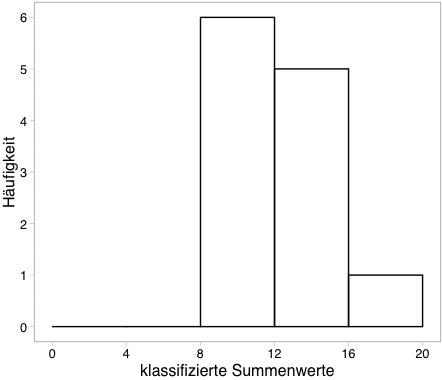
\includegraphics[width=0.8\linewidth]{Anhang/MKHistnn.png}


\end{minipage}
\begin{minipage}{.5\linewidth}
\centering
\raisebox{\depth}
{\begin{tabular}{rrrr}
  \hline
 & absolut & Prozent & kumuliert \\ 
  \hline
(0,4] & 0.00 & 0.00 & 0.00 \\ 
  (4,8] & 0.00 & 0.00 & 0.00 \\ 
  (8,12] & 6.00 & 50.00 & 50.00 \\ 
  (12,16] & 5.00 & 41.67 & 91.67 \\ 
  (16,20] & 1.00 & 8.33 & 100.00 \\ 
   \hline
\end{tabular}

}
%\caption{Häufigkeitstabelle: Fachkompetenz}
\label{tab:defis}
\end{minipage}
\caption{Histogramm und Häufigkeitstabelle der Methodenkompetenz}
\label{fig:MK}
\end{figure}

Wie Tabelle \textasciitilde{}\ref{tab:lMK} zeigt kam der Wert 10 am
häufigsten vor. Mittelwert und Median liegen bei etwa 12,5, was gerade
noch der Klasse 4, also hohem Kompetenzzuwachs entspricht.

\begin{table}[H]
\centering
\caption{Lage- und Streumaße Methodenkompetenz}
\label{tab:lMK}
\begin{tabular}{rrrrrrrr}
  \hline
  N & Minimum & Maximum & Mittelwert & Median & Modus & SD & Varianz \\
  \hline
  12.00 & 10.00 & 17.00 & 12.83 & 12.50 & 10.00 & 2.41 & 5.79 \\
   \hline
\end{tabular}
\end{table}

\begin{itemize}
\tightlist
\item
  Personalkompetenz
\end{itemize}

Der Zuwachs an Personalkompetenz, siehe \textasciitilde{}\ref{fig:PK}
wurde von etwa zwei Drittel der Teilnehmer als hoch eingeschätzt, von
einem Teilnehmer als Mittel und von 3 Teilnehmern als sehr hoch. Es gibt
keine Teilnehmer die keinen oder einen geringen personalen
Kompetenzzuwachs einschätzen.

\begin{figure}[H]
\begin{minipage}{.5\linewidth}
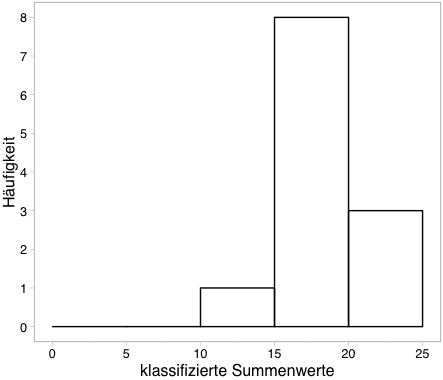
\includegraphics[width=0.8\linewidth]{Anhang/PKHistnn.png}

\label{PK}
\end{minipage}
\begin{minipage}{.5\linewidth}
\centering
\raisebox{\depth}
{\begin{tabular}{rrrr}
  \hline
 & absolut & Prozent & kumuliert \\
  \hline
(0,5] & 0.00 & 0.00 & 0.00 \\
  (5,10] & 0.00 & 0.00 & 0.00 \\
  (10,15] & 1.00 & 8.33 & 8.33 \\
  (15,20] & 8.00 & 66.67 & 75.00 \\
  (20,25] & 3.00 & 25.00 & 100.00 \\
   \hline
\end{tabular}

}
%\caption{Häufigkeitstabelle: Fachkompetenz}
\label{tab:defis}
\end{minipage}
\caption{Histogramm und Häufigkeitstabelle der Personalkompetenz}
\label{fig:PK}
\end{figure}

Mittelwert, Median und Modalwert liegen bei 19, der kleinste Wert
beträgt 11 der höchste Wert 23. Zusammenfassend betrachtet ist auch in
dieser Kategorie der selbsteingeschätzte Kompetenzzuwachs als hoch
einzustufen.

\begin{table}[H]
\centering
\caption{Lage- und Streumaße: Personalkompetenz}
\label{tab:lPK}
\begin{tabular}{rrrrrrrr}
  \hline
  N & Minimum & Maximum & Mittelwert & Median & Modus & SD & Varianz \\
  \hline
  12.00 & 11.00 & 23.00 & 19.17 & 19.00 & 19.00 & 3.04 & 9.24 \\
   \hline
\end{tabular}
\end{table}

\begin{itemize}
\tightlist
\item
  Kommunikationskompetenz
\end{itemize}

\begin{figure}[H]
\begin{minipage}{.5\linewidth}
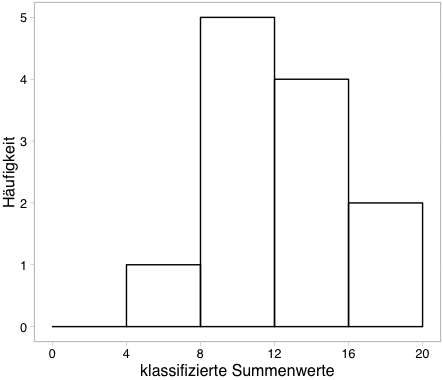
\includegraphics[width=0.8\linewidth]{Anhang/KKHistnn.png}

\label{pic:aufbau}
\end{minipage}
\begin{minipage}{.5\linewidth}
\centering
\raisebox{\depth}
{\begin{tabular}{rrrr}
  \hline
 & absolut & Prozent & kumuliert \\
  \hline
(0,4] & 0.00 & 0.00 & 0.00 \\
  (4,8] & 1.00 & 8.33 & 8.33 \\
  (8,12] & 5.00 & 41.67 & 50.00 \\
  (12,16] & 4.00 & 33.33 & 83.33 \\
  (16,20] & 2.00 & 16.67 & 100.00 \\
   \hline
\end{tabular}

}
%\caption{Häufigkeitstabelle: Fachkompetenz}
\label{tab:defis}
\end{minipage}
\caption{Histogramm und Häufigkeitstabelle der Kommunikationskompetenz}
\
\end{figure}

\begin{table}[H]
\centering
\begin{tabular}{rrrrrrrr}
  \hline
  N & Minimum & Maximum & Mittelwert & Median & Modus & SD & Varianz \\
  \hline
 12.00 & 8.00 & 18.00 & 13.00 & 12.50 & 9,11,16,18 & 3.54 & 12.55 \\

\end{tabular}
\end{table}

\begin{itemize}
\tightlist
\item
  Nutzungsverhalten
\end{itemize}

\begin{figure}[H]
\begin{minipage}{.5\linewidth}
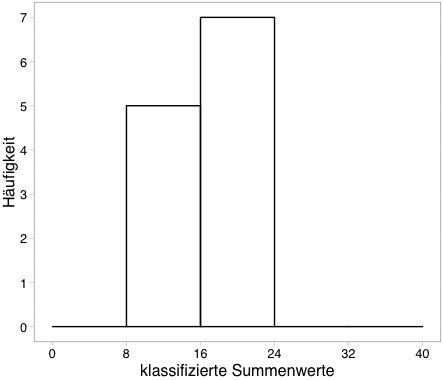
\includegraphics[width=0.8\linewidth]{Anhang/NVHistnn.png}

\label{pic:aufbau}
\end{minipage}
\begin{minipage}{.5\linewidth}
\centering
\raisebox{\depth}
{\begin{tabular}{rrrr}
  \hline
 & absolut & Prozent & kumuliert \\ 
  \hline
(0,8] & 0.00 & 0.00 & 0.00 \\ 
  (8,16] & 5.00 & 41.67 & 41.67 \\ 
  (16,24] & 7.00 & 58.33 & 100.00 \\ 
  (24,32] & 0.00 & 0.00 & 100.00 \\ 
  (32,40] & 0.00 & 0.00 & 100.00 \\ 
   \hline
\end{tabular}

}
%\caption{Häufigkeitstabelle: Fachkompetenz}
\label{tab:defis}
\end{minipage}
\caption{Histogramm und Häufigkeitstabelle des Nutzungsverhaltens}
\end{figure}

\begin{table}[H]
\centering
\begin{tabular}{rrrrrrrr}
  \hline
  N & Minimum & Maximum & Mittelwert & Median & Modus & SD & Varianz \\
  \hline
 12.00 & 9.00 & 21.00 & 16.42 & 17.50 & 14,19 & 3.32 & 10.99 \\     
   \hline
\end{tabular}
\end{table}

\begin{itemize}
\tightlist
\item
  Handlungskompetenz
\end{itemize}

\begin{figure}[H]
\begin{minipage}{.5\linewidth}
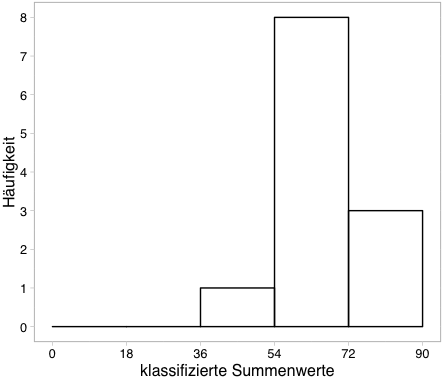
\includegraphics[width=0.8\linewidth]{Anhang/HKHistnn.png}

\label{pic:aufbau}
\end{minipage}
\begin{minipage}{.5\linewidth}
\centering
\raisebox{\depth}
{\begin{tabular}{rrrr}
  \hline
 & absolut & Prozent & kumuliert \\ 
  \hline
(0,18] & 0.00 & 0.00 & 0.00 \\ 
  (18,36] & 0.00 & 0.00 & 0.00 \\ 
  (36,54] & 1.00 & 8.33 & 8.33 \\ 
  (54,72] & 8.00 & 66.67 & 75.00 \\ 
  (72,90] & 3.00 & 25.00 & 100.00 \\ 
   \hline
\end{tabular}

}
%\caption{Häufigkeitstabelle: Fachkompetenz}
\label{tab:defis}
\end{minipage}
\caption{Histogramm und Häufigkeitstabelle der Handlungskompetenz}
\end{figure}

\begin{table}[H]
\centering
\caption{Lage- und Streumaße der Handlungskompetenz}
\begin{tabular}{rrrrrrrr}
  \hline
  N & Minimum & Maximum & Mittelwert & Median & Modus & SD & Varianz \\
  \hline
12.00 & 44.00 & 75.00 & 65.58 & 65.50 & 63,75 & 8.49 & 72.08 \\
   \hline
\end{tabular}
\end{table}

\begin{itemize}
\tightlist
\item
  Handlungskompetenz und Nutzungsverhalten
\end{itemize}

\begin{table}[H]
\centering
\caption{Gesamtkompetenz und Nutzungsverhalten}
\begin{tabular}{rr}
  \hline
 Parameter & Mittelwerte\\
  \hline
Gesamtscore.Kompetenzen & 65.58 \\
  Mittelwert.Kompetenzen & 3.60 \\
  Gesamtscore.Nutzungsverhalten & 16.42 \\
  Mittelwert.Nutzungsverhalten & 2.05 \\
  Gesamtscore.passive.Nutzung & 10.17 \\
  Mittelwert.passive.Nutzung & 2.54 \\
  Gesamtscore.aktive.Nutzung & 6.25 \\
  Mittelwert.aktive.Nutzung & 1.56 \\
   \hline
\end{tabular}
\end{table}

\pagebreak

\pagebreak
\printbibliography
\pagebreak
\appendix


  \section{Anhang}
  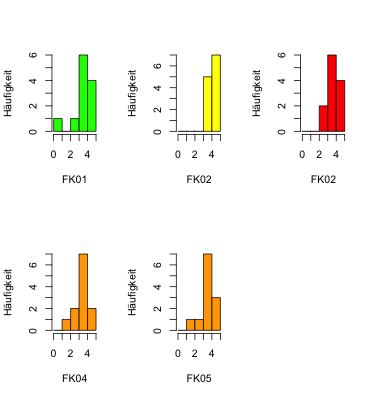
\includegraphics{Anhang/schoen.png}
  %\subsection{Abkürzungen}
  %\renewcommand{\thetable}{{A}.\arabic{table}}
  %\renewcommand{\thetable}{\Alph{section}.\arabic{table}}
  \begin{table}[H]
\centering
%\captionof{table}[Anhang]{Titel}
%\caption{Zuordnung der Items}
\label{itemtabelle}
\resizebox{\textwidth}{!}{%
\begin{tabular}{@{}lllll@{}}
\toprule
Item  & Konstrukt                                                                    & Indikator                                                                                                                                                                           & Ausprägung                                                                                                                                                                                       & Skalenniveau \\ \midrule
1-5   & \begin{tabular}[c]{@{}l@{}}Fach-\\ kompetenz\\FK1,FK2,FK3,FK4,FK5\end{tabular}                    & \begin{tabular}[c]{@{}l@{}}Disposition sachlich-gegenständliche\\ Probleme selbstorganisiert lösen zu können\end{tabular}                                                           & \begin{tabular}[c]{@{}l@{}}5-stufige Likertskala:\\ 1= trifft überhaupt nicht zu\\ 2= trifft wenig zu\\ 3=trifft teils/teils zu\\ 4=trifft überwiegend zu\\ 5=trifft völlig zu\end{tabular}      & metrisch     \\
\midrule
6-10  & \begin{tabular}[c]{@{}l@{}}Methoden-\\ kompetenz\\MK1,MK2,MK3,MK4\end{tabular}                & \begin{tabular}[c]{@{}l@{}}Tätigkeiten und Aufgaben methodisch\\  selbst-organisiert zu gestalten und Methoden\\  weiter zu entwickeln\end{tabular}                                 & \begin{tabular}[c]{@{}l@{}}5-stufige Likertskala: \\ 1= trifft überhaupt nicht zu\\ 2= trifft wenig zu \\ 3=trifft teils/teils zu \\ 4=trifft überwiegend zu \\ 5=trifft völlig zu\end{tabular}  & metrisch     \\
\midrule
11-16 & \begin{tabular}[c]{@{}l@{}}Personal-\\ kompetenz\\PK1,PK2,PK3,PK4,PK5\end{tabular}                & \begin{tabular}[c]{@{}l@{}}Sich einschätzen, selbstorganisiert reflexiv\\  handeln,Werte, Motive und Selbstbilder\\  entwickeln\end{tabular}                                        & \begin{tabular}[c]{@{}l@{}}5-stufige Likertskala: \\ 1= trifft überhaupt nicht zu \\ 2= trifft wenig zu \\ 3=trifft teils/teils zu \\ 4=trifft überwiegend zu \\ 5=trifft völlig zu\end{tabular} & metrisch     \\
\midrule
17-21 & \begin{tabular}[c]{@{}l@{}}Komunikations-\\ kompetenz\\KK1,KK2,KK3,KK4\end{tabular}           & \begin{tabular}[c]{@{}l@{}}Sich mit anderen kreativ auseinander setzen, \\ kommunikativ und selbstorganisiert handeln\\ \parencite[8]{ErpenbeckRosenstiel200305}\end{tabular} & \begin{tabular}[c]{@{}l@{}}5-stufige Likertskala\\ 1= trifft nicht zu,\\2= trifft wenig zu \\ 3=trifft teils/teils zu \\ 4=trifft überwiegend zu \\ 5=trifft vollständig zu\end{tabular}                                                                                    & metrisch     \\
 \midrule
22-28 & \begin{tabular}[c]{@{}l@{}}Nutzungs\\ verhalten\\ Lernplattform NV1,NV2,NV3\\NV4,NV5,NV6,NV7,NV8\end{tabular} & \begin{tabular}[c]{@{}l@{}}Aufschluss über die Intensität u\\ der Nutzung der Lernplattform\end{tabular}                                                                 & \begin{tabular}[c]{@{}l@{}}5-stufige Skala\\ 1=0-1mal genutzt\\ 2=2-4 mal genutzt\\ 3=5-7 mal genutzt\\ 4=8-10 mal genutzt\\ 5=\textgreater10 mal genutzt\end{tabular}                            & metrisch     \\ \bottomrule
\end{tabular}%
}
\end{table}

  \begin{table}[]
\centering
\caption{Einteilung der Klassen}
\label{tab:klassen}
\begin{tabular}{@{}llll@{}}
\toprule
Kompetenz              & Summenwert & Klasse & Bewertung          \\ \midrule
Fach/Personal          & 0-5        & 1      & kein Zuwachs       \\
                       & 5-10       & 2      & geringer Zuwachs   \\
                       & 10-15      & 3      & mittlerer Zuwachs  \\
                       & 15-20      & 4      & hoher Zuwachs      \\
                       & 20-25      & 5      & sehr hoher Zuwachs \\ \cmidrule(r){1-4}
Methoden/Kommunikation & 0-4        & 1      & kein Zuwachs       \\
                       & 4-8        & 2      & geringer Zuwachs   \\
                       & 8-12       & 3      & mittlerer Zuwachs  \\
                       & 12-16      & 4      & hoher Zuwachs      \\
                       & 16-20      & 5      & sehr hoher Zuwachs \\ 
                       \cmidrule(r){1-4}
Handlungskompetenz 	& 0-18       & 1      & kein Zuwachs       \\
                       & 18-36        & 2      & geringer Zuwachs   \\
                       & 36-54       & 3      & mittlerer Zuwachs  \\
                       & 54-72      & 4      & hoher Zuwachs      \\
                       & 72-90      & 5      & sehr hoher Zuwachs \\ 
                       \cmidrule(r){1-4}
Nutzung	& 0-8       & 1      & keine Nutzung       \\
                       & 8-16        & 2      & geringe Nutzung   \\
                       & 16-24       & 3      & mittlere Nutzung  \\
                       & 24-32     & 4      & häufige Nutzung      \\
                       & 32-40      & 5      & sehr häufige Nutzung \\ 
                       \bottomrule
\end{tabular}
\end{table}



%\input{tabelleanalysen}
%\includepdf{alleine.pdf}
\end{document}
